\section{Physical layer software Implementation}
Before implementation is started decisions of which functionalities that will be exposed to the upper layer have to be made. This section will not go into every little aspect of implementing the software, but will give good overview of how the physical layer is utilized and also how it does work internally to process incoming and outgoing data. It is therefore recommended to take a look at the files located at src/physical/ to get the full view of the physical layer. Files that spoken of is listed below:

\begin {itemize}
\item DtmfPhysical.h - This file contain the interface for the implementation of DtmfPhysical class.
\item DtmfPhysical.cpp - This file contain the implementation of DtmfPhysical class.
\item BufferedSoundIO.h - This file contain the interface for the implementation of BufferedSoundIO class.
\item BufferedSoundIO.cpp - This file contain the implementation of BufferedSoundIO class.
\end{itemize}

	\subsection{DtmfPhysical.h - Interface}
	As mentioned the first decisions will define the requirements of the interface. Decisions around the interface are listed below:
	\begin {enumerate}
	\item Constructor have to take parameters for controlling sample rate for incoming and outgoing sound streams, length of sample buffers,
	resolution, and number of channels. All the parameters have to be available for later tweaking purposes.
	\item The interface need to have a send method which take a void pointer as parameter where the frame buffer can be passed as a reference
	so manipulation of the incoming buffer can take place at the physical layer. This is done to avoid copying too much data around in the memory as this task is time consuming.
	\item The interface need to have a receive method which take a void pointer as parameter where the incoming frame buffer for the data link
	layer can be passed as a reference so manipulation of this buffer can take place at the physical layer. This is done for the same reasons as the latter requirement.
	\end{enumerate}
	
	\subsection{DtmfPhysical.cpp - Implementation}
	The interface implementation takes place in the DtmfPhysical class which will be the class for exposing received data to the protocol stack
	and receiving data from the protocol stack for data transmission.
	
	The \textit{constructor} of the physical layer instantiates the BufferedSoundIO which setup PortAudio for utilisation. The constructor passes the
	parameters through the constructor of the BufferedSoundIO.
	
	The \custtt{send(void*)} method takes one parameter as a reference to the buffer exposed from the data link layer to the physical layer. This buffer
	will be of the type \custtt{boost::circular\_ buffer<Frame>}. The \custtt{send} method check if a transmission is going on as \custtt{send} is called.
	If not it resize an internal buffer in the DtmfPhysical so this buffer can hold all frames as one sequence of numbers, the type of 
	the sequence buffer will be \custtt{boost::circular\_buffer <unsigned int>}. This sequence is then pushed to the BufferedSoundIO class which
	internally holds a buffer of the same type. A simple flowchart of the \custtt{send} method is shown in figure \ref{fig:physical_send}.
	
	\begin{figure}[htb]
		\begin{center}
		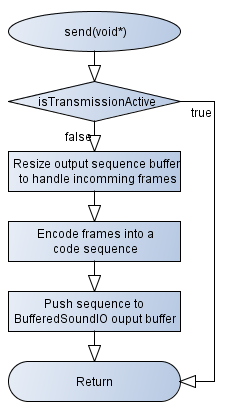
\includegraphics[scale=0.66,trim=0 0 0 0]{physical_send.png}%trim=l b r t
		\caption{An overview of the internal workings in the \smalltt{send} method}
		\label{fig:physical_send}
		\end{center}
	\end{figure}
	
	The \custtt{receive(void*)} method takes one parameter as a reference to the buffer which stores data for link layer is delivered from the physical layer.
	This buffer	will be of the type \custtt{boost::circular\_buffer<Frame>}. The \custtt{receive} method check if the internal frame buffer is empty.
	If this is not the case the frames are delivered up to the data link layer. A simple flowchart of the \custtt{receive} method is shown in figure \ref{fig:physical_receive}.
	
	\begin{figure}[htb]
		\begin{center}
		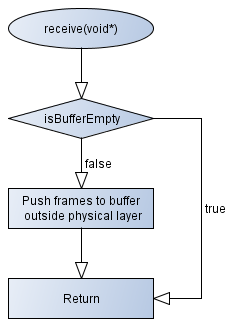
\includegraphics[scale=0.66,trim=0 0 0 0]{physical_receive.png}%trim=l b r t
		\caption{Flowchart shown here gives an overview of the internal workings in the \smalltt{receive} method.}
		\label{fig:physical_receive}
		\end{center}
	\end{figure}
	
	\subsection{Internal workings of the BufferedSoundIO}
	The interface of BufferedSoundIO will not be explained in greater detail as the instantiation is handled by the DtmfPhysical class.
	
	The DtmfPhysical class is fairly simple compared to the BufferedSoundIO class. This is because BufferedSoundIO have to control two processes
	at the same time which are fired by PortAudio.
	
	\begin{enumerate}
	\item Output streaming
	\item Input streaming
	\end{enumerate}
	
	To understand BufferedSoundIO a little knowledge of how PortAudio works internally is needed. PortAudio provides the user of the API to initialize
	and start a sound stream through a computers sound card. This stream \textit{of sound} or data is available through a callback function delivered
	by PortAudio. As PortAudio is programmed in C, this callback function is simply a function pointer\footnote{\url{http://www.newty.de/fpt}}
	which allow for the user to create a function in his program that will be called when PortAudio is calling its own callback function.
	This callback is called according to the setup of a given stream, for instance, if the sample rate is $8kHz$ and the stream is initialized as 
	only output with a buffer of 8000 samples, then this stream will fire the callback every second as the buffer is emptied every second.
	The same goes for input streams but a little different, every time the input buffer is full the stream callback is fired. To implement
	this type of function a well defined pattern have to be followed, the pattern is defined by PortAudio and come in the form of a
	function declaration with an arbitrary name. 
	
	\begin{lstlisting}[float=htb,language={C++},caption={PortAudios callback function declaration. This declaration is used for both input
	streams, output streams, and the two in combination},label={lst:pa_callback}]
static int paStreamCallback(const void *inputBuffer,
							void *outputBuffer,
							unsigned long framesPerBuffer,
							const PaStreamCallbackTimeInfo* timeInfo,
							PaStreamCallbackFlags statusFlags,
							void *userData);
	\end{lstlisting}
	
	BufferedSoundIO is instantiated with DtmfPhysical and therefore resides in DtmfPhysical. BufferedSoundIO itself setup two streams where each
	represent either a input or output stream, this is done because the physical layer works on two streams of data seperately. As two streams are 
	now present, a foundation for communication with sound is founded. These two streams are able to work asynchronously which might proof to be an
	advantage later on. If the input callback is fired twice as often as the output callback, could proof to make the communication more reliable
	as this could address some of the overlapping issues which could lead to loss of data. Exact scientific tests on the topic will not be performed
	due to time constraints, but a rule of thumb is, be sure to fire the input callback at least twice as often as the output callback.
	
		\subsubsection{Output streaming}
		The output stream fires the internal \custtt{paOutputStreamCallback} function of BufferedSoundIO. As shown in listing \ref{lst:pa_callback}
		the last parameter taken by PortAudio callback \custtt{void *userData} is used so the user is able to pass arbitrary data as a reference into the
		callback. Regarding BufferedSoundIO this parameter is used to send a reference to the object itself in which the stream resides. 
		Listing \ref{lst:pa_stream_callback} show the exact implementation of \custtt{paOutputStreamCallback}.
		
		\begin{lstlisting}[float=htb,language={C++},caption={Implementation of \smalltt{paOutputStreamCallback}},label={lst:pa_stream_callback}]
static int paOutputStreamCallback(	const void *inputBuffer,
									void *outputBuffer,
									unsigned long framesPerBuffer,
									const PaStreamCallbackTimeInfo* timeInfo,
									PaStreamCallbackFlags statusFlags,
									void *userData)
{ return ((BufferedSoundIO*)userData) -> outputStreamCallback(inputBuffer, outputBuffer, framesPerBuffer, timeInfo, statusFlags); }
		\end{lstlisting}
		
		This way of implementing the callback makes the callback able to reach data which resides in the object of BufferedSoundIO,
		\custtt{paOutputStreamCallback} call the \custtt{outputStreamCallback} which is also a member function of BufferedSoundIO.
		
		The \custtt{outputStreamCallback(...)} essentially generate sound according to entries in an internal buffer of BufferedSoundIO
		if there is any present, a sketch up of the flowchart of \custtt{outputStreamCallback(...)} is shown in Figure \ref{fig:physical_output_callback}.
		
		\begin{figure}[htb]
			\begin{center}
			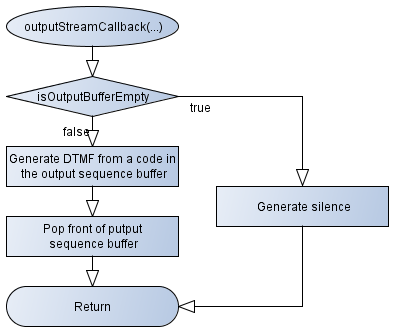
\includegraphics[scale=0.66,trim=0 0 0 0]{physical_output_callback.png}%trim=l b r t
			\caption{A sketch up of \smalltt{outputStreamCallback(...)} function. For more details this can be found in BufferedSoundIO.cpp}
			\label{fig:physical_output_callback}
			\end{center}
		\end{figure}
		
		\subsubsection{Input streaming}
		Input streaming works in the exact same way as the output stream regarding the callback. BufferedSoundIO have a function named
		\custtt{paInputStreamCallback} which handles the callback from PortAudio, \custtt{paInputStreamCallback} call the \custtt{inputStreamCallback}
		function which handles the internal input buffer exposed by PortAudio. Figure \ref{fig:physical_input_callback} show a sketch up of \custtt{inputStreamCallback}.
		
		This function is a little more complex compared to the output callback as this implements the Goertzel algorithm for detection of tones and also
		a decision making system which analyse the state of the signal to see if it is a valid signal. If the signal is valid a code is calculated, this
		code is now validated to see if it is contained in the mapping system of tones and codes. If the code is valid it is pushed to the input
		sequence buffer which is of the type \custtt{boost::circular\_buffer<unsigned int>}. When ever the decision making system see the code 17,
		which corresponds to end of a frame a callback is made from BufferedSoundIO to DtmfPhysical asking the DtmfPhysical to pull the codes from
		the input sequence buffer which is held in BufferedSoundIO.
		
		\begin{figure}[htb]
			\begin{center}
			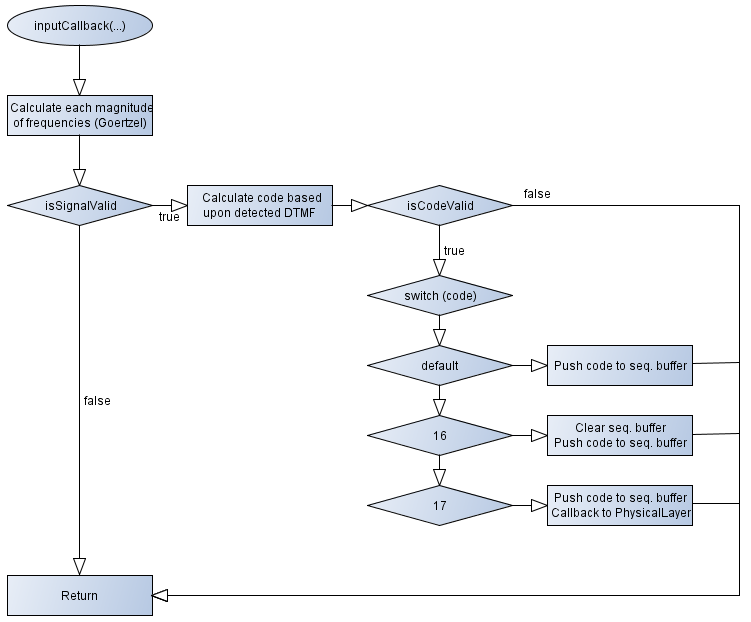
\includegraphics[scale=0.66,trim=0 0 0 0]{physical_input_callback.png}%trim=l b r t
			\caption{A sketch up of \smalltt{inputStreamCallback(...)} function. For more details this can be found in BufferedSoundIO.cpp}
			\label{fig:physical_input_callback}
			\end{center}
		\end{figure}
		
	\subsection{Callback to DtmfPhysical}
	Everytime the input callback in BufferedSoundIO recognise the code 17, a callback is made back to the DtmfPhysical. This callback pull the
	codes from BufferedSoundIO, generate a frame from the information pulled, and store this frame in the frame buffer of DtmfPhysical. This ensures
	that frames and the functionality for generating sequences from frames and generating frames from sequences are kept in the DtmfPhysical class.
	A sketch up of the function is shown in figure \ref{fig:physical_frame_callback}
	
	\begin{figure}[htb]
		\begin{center}
		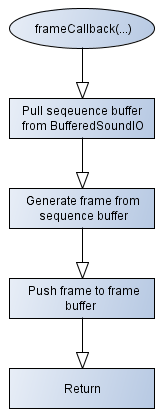
\includegraphics[scale=0.6,trim=0 0 0 0]{physical_frame_callback.png}%trim=l b r t
		\caption{A sketch up of \smalltt{frameCallback(...)} function.}
		\label{fig:physical_frame_callback}
		\end{center}
	\end{figure}
